\documentclass[dvipdfmx]{jsarticle}

\title{個人レベルでGithubを使う}
\author{Seiichi Nukayama}
\date{2021-07-09}
\usepackage{tcolorbox}
\usepackage{color}
\usepackage{listings, plistings}

% Java
\lstset{% 
  frame=single,
  backgroundcolor={\color[gray]{.9}},
  stringstyle={\ttfamily \color[rgb]{0,0,1}},
  commentstyle={\itshape \color[cmyk]{1,0,1,0}},
  identifierstyle={\ttfamily}, 
  keywordstyle={\ttfamily \color[cmyk]{0,1,0,0}},
  basicstyle={\ttfamily},
  breaklines=true,
  xleftmargin=0zw,
  xrightmargin=0zw,
  framerule=.2pt,
  columns=[l]{fullflexible},
  numbers=left,
  stepnumber=1,
  numberstyle={\scriptsize},
  numbersep=1em,
  language={Java},
  lineskip=-0.5zw,
  morecomment={[s][{\color[cmyk]{1,0,0,0}}]{/**}{*/}},
}
\usepackage{url}
% \usepackage[dvipdfmx]{graphicx}
\usepackage[dvipdfmx]{hyperref}
\usepackage{amsmath, amssymb}
\usepackage{itembkbx}
\usepackage{eclbkbox}	% required for `\breakbox' (yatex added)
\usepackage{enumerate}
\usepackage{setspace}
\fboxrule=0.5pt
\parindent=1em
\begin{document}

%\anaumeと入力すると穴埋め解答欄が作れるようにしてる。\anaumesmallで小さめの穴埋めになる。
\newcounter{mycounter} % カウンターを作る
\setcounter{mycounter}{0} % カウンターを初期化
\newcommand{\anaume}[1][]{\refstepcounter{mycounter}{#1}{\boxed{\phantom{aa}\themycounter \phantom{aa}}}} %穴埋め問題の空欄作ってる。
\newcommand{\anaumesmall}[1][]{\refstepcounter{mycounter}{#1}{\boxed{\tiny{\phantom{a}\themycounter \phantom{a}}}}}%小さい版作ってる。色々改造できる。

%% 修正時刻: Fri Jul  9 12:01:07 2021


\section{Eclipseで Github を使う}

\subsection{ワークスペースをGitで管理する}

\subsubsection{ワークスペース名の決定}

\textsf{C:}ドライブの直下にワークスペースを作成し、それをGitで管理することにする。

ワークスペース名: \textsf{workspace\_git}

\subsubsection{Githubでリポジトリを作成する}

Githubにサインインして、新しいリポジトリを作成する。

% 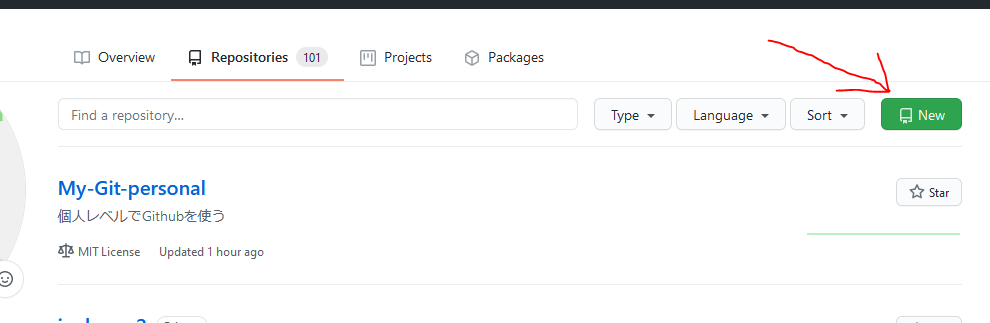
\includegraphics[width=10cm]{img/11newRepo.png}

\textsf{NEW}をクリックして始める。

\textsf{Create a new repository} の画面が開く。

\vspace{3mm}
\fbox{\textsf{Repository name}}

まず、リポジトリ名を入力する。今回は \textsf{workspace\_git} とした。

Description には、このリポジトリの簡単な説明を入れておく。
今回は、「git用ワークスペース」としておく。

% 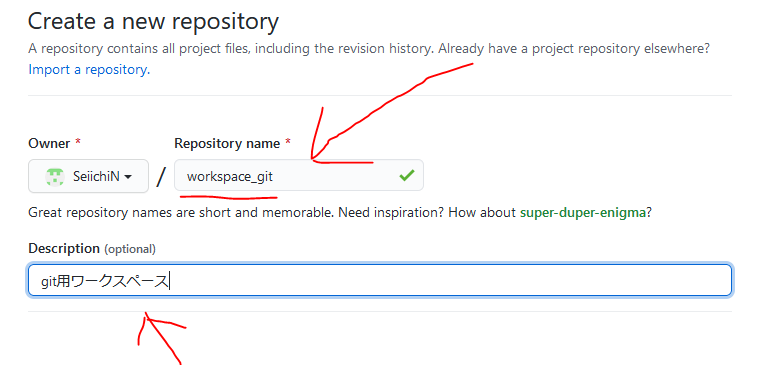
\includegraphics[width=10cm]{img/12repoName.png}

\vspace{3mm}
\fbox{\textsf{Public / Private}}

このリポジトリを公開するかどうかを設定する。今回は \textsf{Private} とする。

\vspace{3mm}
\fbox{\textsf{Add a README fle}}

README.md というファイルを作成するかどうかだが、作成しておいたほうが何かと便利。

\vspace{3mm}
\fbox{\textsf{Add .gitignore}}

.gitignore というファイルを作成するかどうかだが、これも作成しておいたほうが便利。

これにチェックを入れると、入力欄が表示される。ここでは \textsf{Java} を選択しておく。

\vspace{3mm}
\fbox{\textsf{Choose a license}}

どういうライセンスにするかを選択できる。今回は Private すなわち非公開なので、
選択しなくてもかまわない。

ちなみに一番ゆるいライセンスは、MITライセンス。

\vspace{3mm}
\fbox{\textsf{Create repository}} ボタンをクリックすると、リポジトリが作成される。

\vspace{3mm}
新しくできたリポジトリの画面が表示される。\fbox{Code} ボタンをクリックする。

\textsf{https://github.com/xxxxxx/workspace\_git.git} が表示されるので、
コピーしておく。(コピーボタンがあるので、それをクリック)


\subsubsection{クローンする}

今回は、C:ドライブ直下に Git用ワークスペースを作成したいので、
C:ドライブで コマンドプロンプトを開く。

\verb!C:> ! と表示されるので、\textsf{git clone } と入力してから、
Ctrl-v として、先ほどコピーしておいたものを貼り付ける。

\begin{tcolorbox}
\verb!C:> git clone https://github.com/xxxxxx/workspace_git.git!
\end{tcolorbox}

これで、C:ドライブに \textsf{workspace\_git} というフォルダが作成されている。

\subsubsection{Eclipseでそのワークスペースで作業する}

Eclipseを起動して、その今作成したワークスペースを指定する。

そして、そこで何らかのプロジェクトを作成し、コードを書く。

今回は、\textsf{sample} という Javaプロジェクトを作成し、
\textsf{src} に \textsf{Main.java} というクラスを作成して、
以下のコードを書いた。

\begin{lstlisting}[caption=Main.java]
public class Main {
  public static void main(String[] args) {
    System.out.println("テスト");
  }
}
\end{lstlisting}

\subsubsection{.gitignoreファイルを修正する}

\textsf{.gitignore}というファイルで、どのファイル・フォルダをGitで同期するかを
指定できる。
今回は以下のように設定した。

\begin{lstlisting}[caption=.gitignore]
 # Compiled class file
 *.class

 # Log file
 *.log

 # BlueJ files
 *.ctxt

 # Mobile Tools for Java (J2ME)
 .mtj.tmp/

 # Package Files #
 *.jar
 *.war
 *.nar
 *.ear
 *.zip
 *.tar.gz
 *.rar

 # virtual machine crash logs, see http://www.java.com/en/download/help/error_hotspot.xml
 hs_err_pid*
 /.metadata/

 # add by Seiichi --------------------- <1>
 /Servers/
 .settings/
 build/
 bin/
 .classpath
 .project
 META-INF/

 # necessary
 !jstl-api-1.2.jar
 !jstl-impl-1.2.jar
 \end{lstlisting}

 \verb!<1>! までの記述は、GitHubが自動で書いてくれたものである。

 今回書いたのは、\verb!<1>! 以下である。
 ここに書いたファイルやフォルダは同期の対象から外すことができる。

 また、先頭に \verb|!| のついているものは、同期を外すの反対なので、同期させるという意味である。
 
 
\subsubsection{ワークスペースの変更をGithubに反映させる}

\verb!C:\workspace_git! でコマンドプロンプトを開く。

\begin{tcolorbox}
 \verb!> git status!
\end{tcolorbox}

とすると、どのファイル・フォルダが新しく追加されたか、あるいは変更されたかを表示してくれる。

\begin{tcolorbox}
\begin{verbatim}
C:\workspace_git>git status
On branch main
Your branch is up to date with 'origin/main'.

Changes not staged for commit:
  (use "git add <file>..." to update what will be committed)
  (use "git restore <file>..." to discard changes in working directory)
        modified:   .gitignore

Untracked files:
  (use "git add <file>..." to include in what will be committed)
        sample/

no changes added to commit (use "git add" and/or "git commit -a")    
\end{verbatim}
\end{tcolorbox}

また、\verb!-u! オプションをつけると、フォルダの中のファイルも表示してくれる。

\begin{tcolorbox}
 \verb!> git status -u! 
\end{tcolorbox}

以下のようになる。

\begin{tcolorbox}
\begin{verbatim}
C:\workspace_git>git status -u
On branch main
Your branch is up to date with 'origin/main'.

Changes not staged for commit:
  (use "git add <file>..." to update what will be committed)
  (use "git restore <file>..." to discard changes in working directory)
        modified:   .gitignore

Untracked files:
  (use "git add <file>..." to include in what will be committed)
        sample/src/Main.java

no changes added to commit (use "git add" and/or "git commit -a")    
\end{verbatim}
\end{tcolorbox}
\footnote{
 もし、.gitignoreを修正しなかったら、以下のようになる。\\
 ------------------------------------------------------ \\
 Changes not staged for commit: \\
   (use "git add $<$file$>$..." to update what will be committed) \\
   (use "git restore $<$file$>$..." to discard changes in working directory) \\
         modified:   .gitignore  \\
 \\
 Untracked files: \\
   (use "git add $<$file$>$..." to include in what will be committed) \\
         sample/.classpath \\ 
         sample/.project \\
         sample/.settings/org.eclipse.jdt.core.prefs \\
         sample/src/sample/Main.java  \\
 \\
 no changes added to commit (use "git add" and/or "git commit -a")    \\
 ------------------------------------------------------ \\
 この場合、Eclipseでのプロジェクトの設定情報まで同期することになる。
 そうなると、いろいろややこしいことになるので、ここでは
 srcフォルダなどのソース・フォルダのみ同期することにしている。
}

また、このとき、1行目の \textsf{On branch main} と
2行目の \textsf{Your branch is up to date with 'origin/main'.} にも
注意を払っておく。

これは、「現在、''main'' というブランチ(枝)で作業していますよ。」

「あなたのブランチは、 ''origin'' の ''main'' ですよ。」 という意味である。

''origin'' というのは、今回の場合は、
\begin{tcolorbox}
 \verb!https://github.com/xxxxxx/workspace_git.git!
\end{tcolorbox}
のことで(この URL の別名)、''main'' というのは、このソース群に github がつけた
\textgt{ブランチ名} である。
\footnote{ブランチは開発者が、たとえば textsf{ver2} などとつけることができる。
たとえば、\textsf{main} での開発はできた。今度はこの機能を追加したバージョンを
作成してみよう。今度の新バージョン開発ブランチを \textsf{ver2} としよう。
そして、\textsf{main} ブランチから \textsf{ver2} ブランチに切り換えて開発を行うことにしよう。
そうすることで、\textsf{main} ブランチの保守作業もできるし、\textsf{ver2} での開発も同時に
できるというわけである。}
\footnote{\textsf{main}というのは最近になって GitHub が使うようになった
デフォルト・ブランチ名である。それまでは、\textsf{master} がデフォルト・ブランチ名だった。}


\subsubsection{変更ファイルを指定する}

変更・追加したファイルをローカル・リポジトリ(このプロジェクトの保管場所。今作業しているフォルダの中に作成されている)に追加する。これを\textgt{ステージング}という。

\begin{tcolorbox}
 \verb!> git add .! (ピリオド)
\end{tcolorbox}

この \textsf{.} (ピリオド) は、ここにあるものすべて、という意味であるが、変更・追加・削除
のあったものを指定したことになる。変更のなかったものは含まれない。

\subsubsection{変更を確定し、説明文をつける}

次に、この変更を確定する。このときに必ず説明文をつけなくてはならない。
これは当然で、この変更追加は何のためなのか、どういう変更なのかを説明しなければ、
他の人に伝わらないし、また、自分があとで見ても、説明がなければ理解できない。

\begin{tcolorbox}
 \verb!> git commit -m "Main.javaを新しく追加"!
\end{tcolorbox}

\begin{tcolorbox}
 workspace\_git> git commit -m ``Main.javaを新しく追加''
 [main fda8839] Main.javaを新しく追加
 3 files changed, 27 insertions(+)
 create mode 100644 sample/.gitignore
 create mode 100644 sample/src/Main.java
\end{tcolorbox}

\subsubsection{ネット上の GitHub リポジトリと同期する}

これでローカル・リポジトリは新しくなった。
しかし、インターネット上に作成した リポジトリ(リモート・リポジトリという)は古いままである。
今からリモート・リポジトリを更新する。

以下のコマンドで更新できる。

\begin{tcolorbox}
 \verb!> git push -u origin main!
\end{tcolorbox}

ここで \textsf{-u} オプションをつけているのは、のちに出てくる \textsf{git fetch} コマンドで
 \textsf{origin} の指定を省略できるようにするためである。

以下のように出力されると成功である。

\begin{tcolorbox}
\begin{verbatim}
 workspace_git> git push -u origin main
 Enumerating objects: 9, done.
 Counting objects: 100% (9/9), done.
 Delta compression using up to 8 threads
 Compressing objects: 100% (5/5), done.
 Writing objects: 100% (7/7), 776 bytes | 776.00 KiB/s, done.
 Total 7 (delta 1), reused 0 (delta 0)
 remote: Resolving deltas: 100% (1/1), completed with 1 local object.
 To https://github.com/SeiichiN/workspace_git.git
 1ece74f..fda8839  main -> main
 Branch 'main' set up to track remote branch 'main' from 'origin'.
\end{verbatim}
\end{tcolorbox}

ここで \textsf{git log} として、うまくプッシュできたかを確認する。

\begin{tcolorbox}
\begin{verbatim}
 workspace_git> git log
 commit fda8839f98b074ab6e449912f2014a4c790faf05 (HEAD -> main, origin/main, orig
 in/HEAD)
 Author: SeiichiN <billie175@gmail.com>
 Date:   Mon Jul 12 16:23:27 2021 +0900

 Main.javaを新しく追加
\end{verbatim}
\end{tcolorbox}    


\subsection{別のPCで作業を再開する}

たとえば、自宅のデスクトップPCで作業をし、それを GitHub にプッシュしておいたとする。
その作業の続きを、出先のノートパソコンでおこなうことにする。

\subsubsection{Gitクローンする}

ノートパソコンの適当なフォルダでコマンド・プロンプトを開き、そこで git clone とする。
ここでは、デスクトップでやったときと同じように、\verb!C:!ドライブのトップに
ワークスペースを作成することにする。

あらかじめ、ブラウザで GitHubのページを開き、\textsf{Code} ボタンをクリックして、
クローンするための URL をコピーしておく。

それから、\verb!C:!ドライブのトップでコマンド・プロンプトを開き、以下のコマンドを
実行する。

\begin{tcolorbox}
\begin{verbatim}
 > git clone https://github.com/xxxxxx/workspace_git
\end{verbatim} 
\end{tcolorbox}

\subsubsection{Eclipseで新規プロジェクト}

Eclipseを起動する。ワークスペースにクローンしておいた \textsf{workspace\_git} を
指定する。

新規でプロジェクトを作成する。

このとき注意することは、デスクトップPCで作成したプロジェクト名と同じ名前を指定
することである。

すると、クローンしておいたファイルが自動で読み込まれる。
今回の例でいうと、\textsf{src} フォルダの中の \textsf{Main.java} が自動的に
読み込まれる。

ここで、Main.java を修正したり、他のファイルを追加したりする。

\subsubsection{GitHubにプッシュ}

以下の作業をして、GitHubにプッシュする。

\begin{tcolorbox}
\begin{verbatim}
 > git status
 > git add .
 > git commit -m "Main.javaを修正"
 > git push -u origin main
 > git log    
\end{verbatim} 
\end{tcolorbox}


\subsection{もとのPCで作業を再開する}

最初のPCで作業を再開することにする。

出先のノートパソコンで変更を加えているので、まず、それをとりこまねばならない。

Eclipseを 開く前に、Gitで管理しているワークスペースをコマンドプロンプトで 開く。

\begin{tcolorbox}
 $>$ cd c:\yen workspace\_git \\
 C:\yen workspace\_git$>$
\end{tcolorbox}

まず、リモート・リポジトリ(github.com/xxxxxx/workspace\_git)に変更があるかを問い合わせる。

\begin{tcolorbox}
 C:\yen workspace\_git$>$ \textsf{git fetch}
\end{tcolorbox}

変更がある場合、以下のような表示になる。

\begin{tcolorbox}
\begin{verbatim}
 workspace_git> git fetch
 remote: Enumerating objects: 9, done.
 remote: Counting objects: 100% (9/9), done.
 remote: Compressing objects: 100% (2/2), done.
 remote: Total 5 (delta 2), reused 5 (delta 2), pack-reused 0
 Unpacking objects: 100% (5/5), 451 bytes | 451.00 KiB/s, done.
 From https://github.com/xxxxxx/workspace_git
 fda8839..4ee1984  main       -> origin/main
\end{verbatim}
\end{tcolorbox}

ここで git status とする。

\begin{tcolorbox}
 $>$ git status
\end{tcolorbox}

以下のような表示になる。

\begin{tcolorbox}
\begin{verbatim}
workspace_git> git status
ブランチ main
このブランチは 'origin/main' に比べて1コミット遅れています。fast-forwardすることができます。
  (use "git pull" to update your local branch)

  nothing to commit, working tree clean
\end{verbatim}
\end{tcolorbox}

ここで、\textsf{use ``git pull'' to update your local branch} と表示されているのを確認する。

「あなたのローカル・ブランチを更新するには ``git pull'' しなさい」という意味(私訳)

そのとおりにする。

\begin{tcolorbox}
 $>$ git pull
\end{tcolorbox}

以下のような表示になる。

\begin{tcolorbox}
\begin{verbatim}
workspace_git> git pull
Updating fda8839..4ee1984
Fast-forward
 sample/src/Main.java | 4 ++--
  1 file changed, 2 insertions(+), 2 deletions(-)
\end{verbatim}
\end{tcolorbox}

これで、このフォルダは更新されている。また、git log とすることで、
メッセージを確認できる。

\begin{tcolorbox}
\begin{verbatim}
workspace_git> git log
commit 4ee1984640c5c710d025b25eff46a1c15ede52ec (HEAD -> main, origin/main, ori
gin/HEAD)
Author\hline SeiichiN <billie175@gmail.com>
Date\hline   Mon Jul 12 19\hline10\hline06 2021 +0900

    Main.javaを修正

commit fda8839f98b074ab6e449912f2014a4c790faf05
Author: SeiichiN <billie175@gmail.com>
Date:   Mon Jul 12 16:23:27 2021 +0900

    Main.javaを新しく追加
( ... 略 ...)
\end{verbatim}
\end{tcolorbox}


これで更新できたので、Eclipseを起動し、プロジェクトを開いて、編集をおこなう。

編集がすめば、また、workspace\_git のフォルダにて、以下のコマンドを実行して
リモート・リポジトリに変更を同期させる。

\begin{tcolorbox}
 $>$ git status \\
 $>$ git add . \\ 
 $>$ git commit -m ``変更点を簡潔に記述する'' \\
 $>$ git push -u origi main \\
 $>$ git log \\
\end{tcolorbox}

出先のノートパソコンで 作業の続きをおこなうには、前回ですでにワークスペースは
クローンできているので、以下のように作業できる。

\begin{tcolorbox}
 $>$ cd C:\yen workspace\_git \\
 $>$ git fetch \\
 $>$ git status \\
 $>$ git pull \\
 $>$ git log \\
\end{tcolorbox}
        

    
\end{document}

%% 修正時刻: Sat May  2 15:10:04 2020


%% 修正時刻: Mon Jul 12 19:42:36 2021
